\chapter{Algorithm}



Electron backscatter diffraction (EBSD) is a scientific tool used to examine crystalline materials. The principle of EBSD is sketched in \cref{ebsd-principle}. It is based on electron diffraction: when a beam of electrons is emitted towards the specimen, some of the electrons backscatter. They are then reflected on phosphor screen which is coupled with compact lens that directs the captured image towards a camera. The result of the procedure is a grayscale image of the \emph{electron backscatter pattern} (EBSP). An example of EBSP is shown in \cref{ebsp-example}.

The electrons do not reflect randomly, but based on the examined specimen, they backscater in a specific way, forming \emph{Kukuchi lines} observable in the EBSP. The geometry of Kukuchi lines can be interpreted as a projection of the specimen crystal structure on the flat phosphor screen.

When 


EBSD is used with scanning electron microscope. 

\begin{figure}
	\centering
	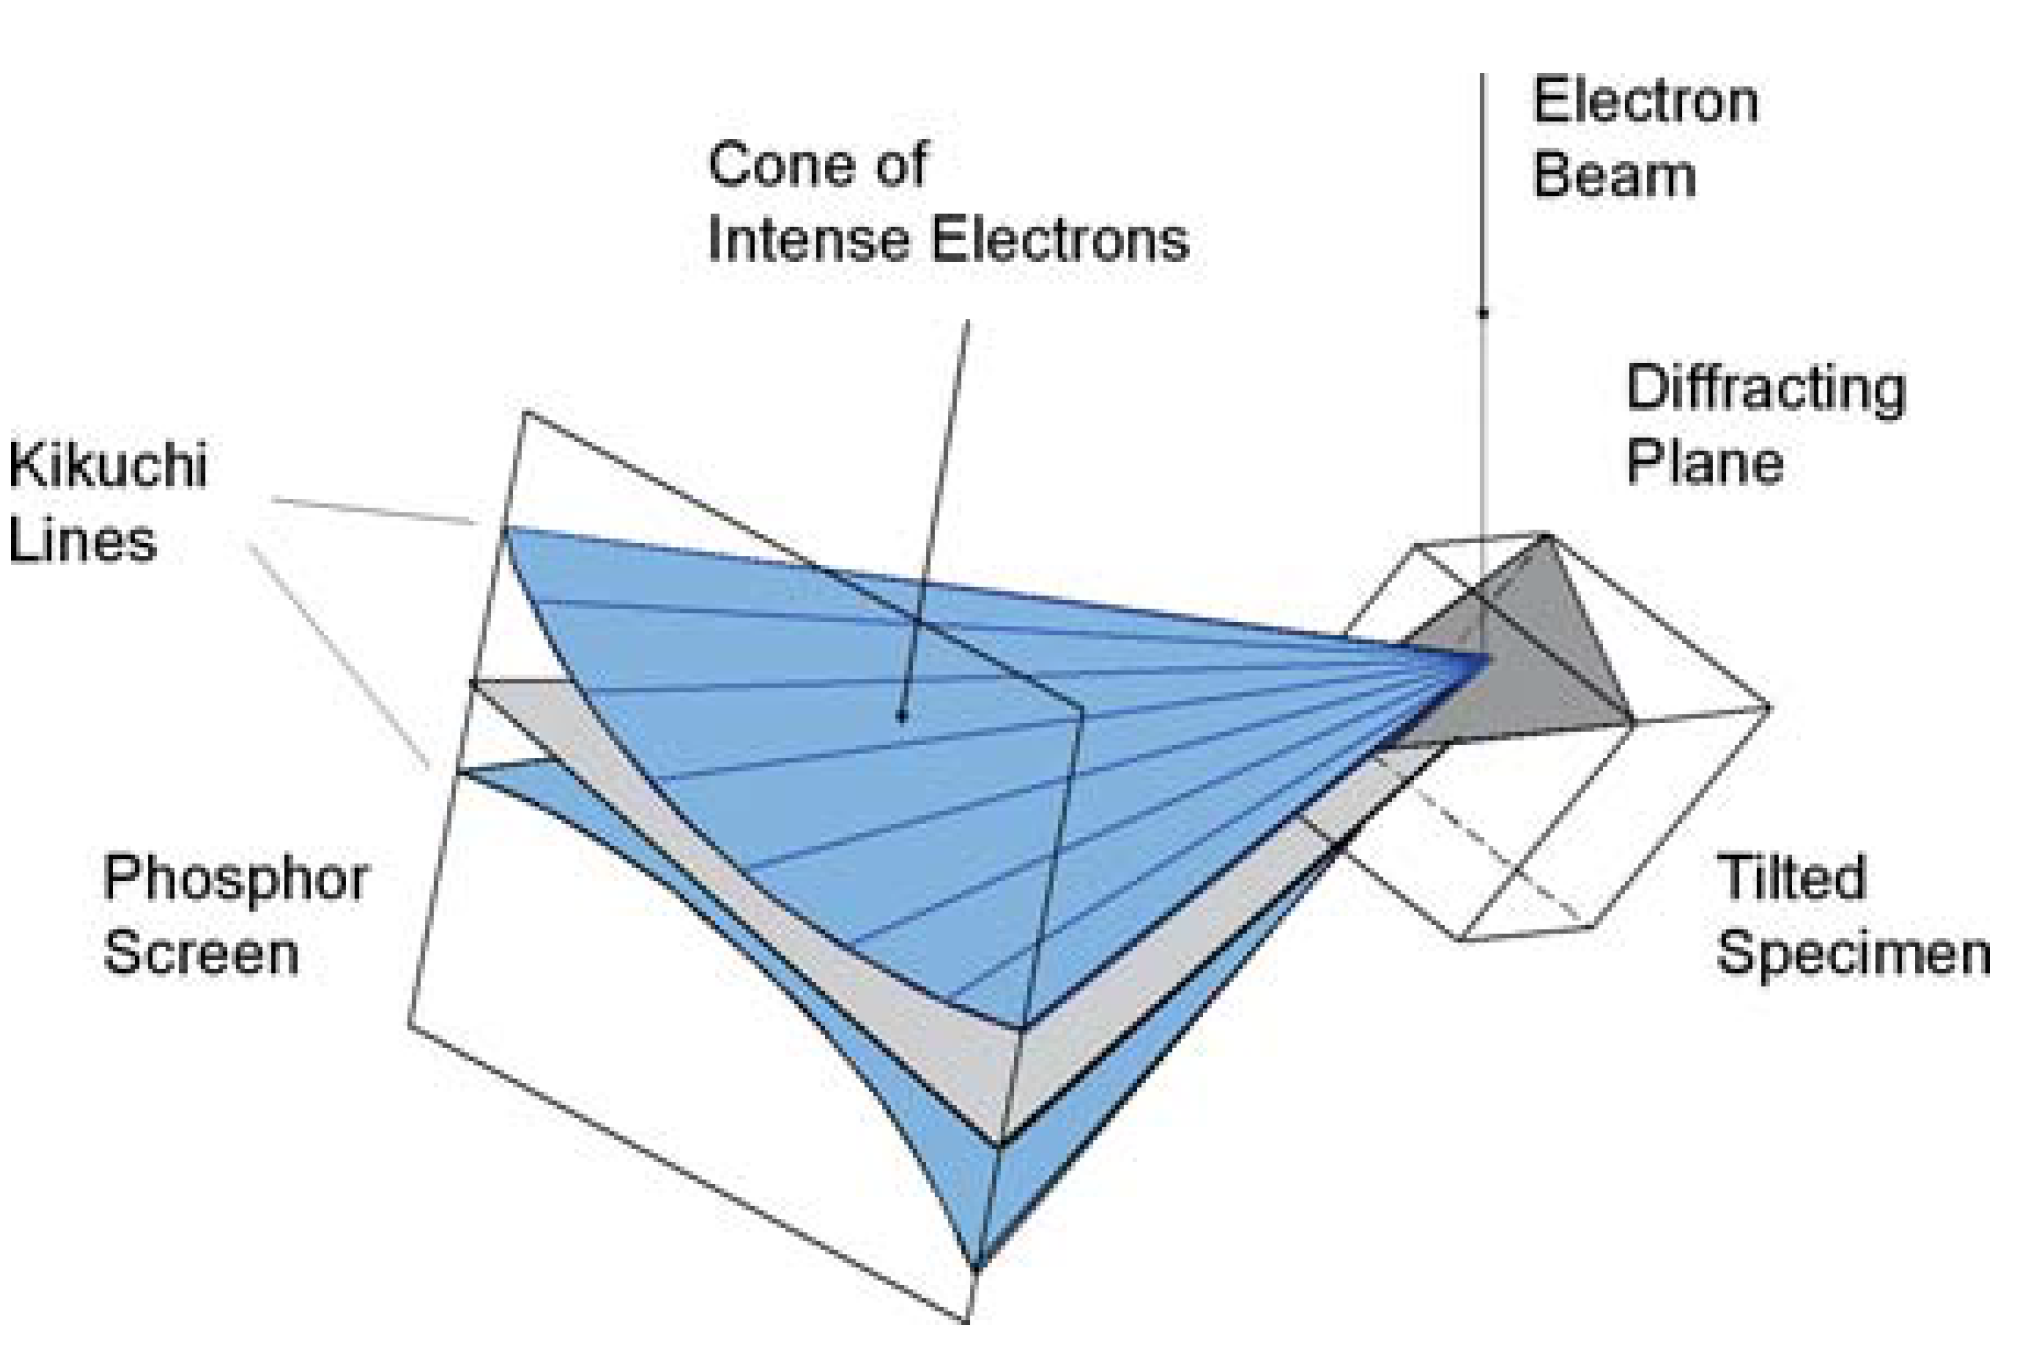
\includegraphics[width=0.9\textwidth]{img/ebsd_principle}
	\caption{The principle of EBSD. The image is taken from \cite{schwartz2009electron}.}
	\label{ebsd-principle}
\end{figure}

\begin{figure}
	\centering
	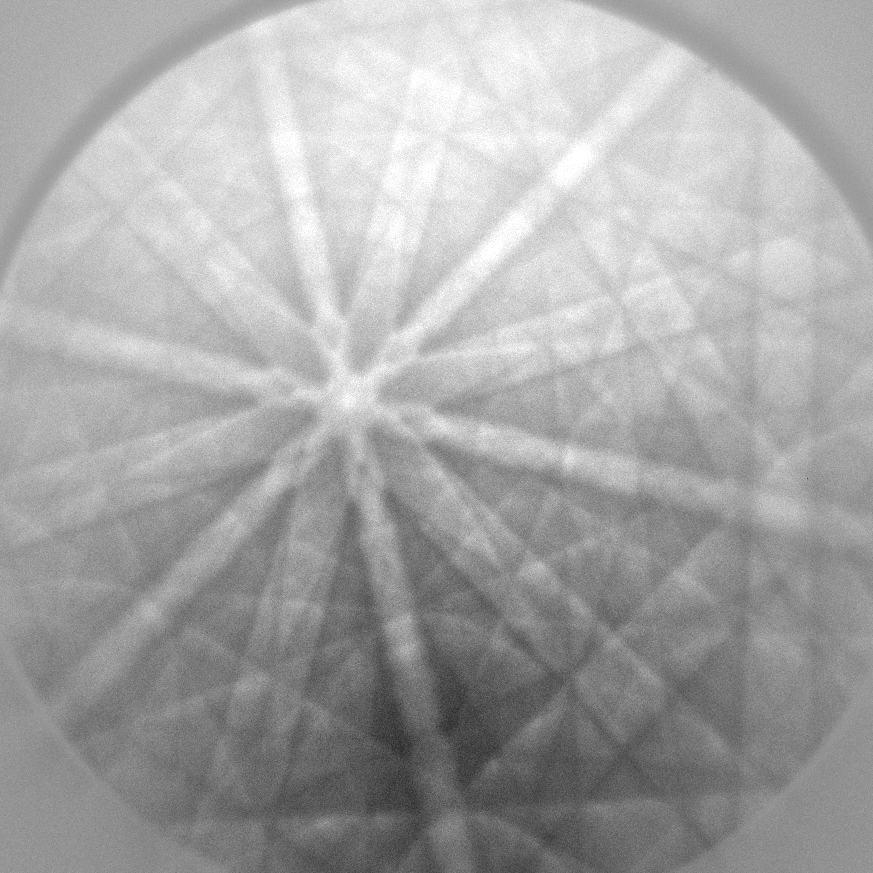
\includegraphics[width=0.7\textwidth]{img/INITIAL_x0y0}
	\caption{Electron backscatter pattern of the FeAl compound.}
	\label{ebsp-example}
\end{figure}


\section{Title of the first subchapter of the first chapter}

